\section{Modelado y simulación de un sistema térmico por analogía con un circuito eléctrico}
\subsection{Diseño y modelización} \label{modelado}
\begin{enumerate}
   \item Utilizando la analogía de los sistemas eléctricos, modelar matemáticamente el sistema correspondiente al circuito mostrado en la figura 1, que representa un dispositivo electrónico de potencia sin disipador.
   \item En la práctica y para poder garantizar condiciones operativas seguras se utilizan disipadores, tal como se plantea en la introducción. Desarrollar el circuito térmico equivalente para un dispositivo electrónico de potencia con disipador. Identificar en forma clara el circuito implementado y modelar matemáticamente el sistema propuesto.
\end{enumerate}
\subsubsection{Resolución}
Los circuitos eléctricos pueden utilizarse para modelar problemas de conducción de calor. Esta analogía consiste en tratar a la temperatura
como si fueran diferencias de potencial eléctrico, a los flujos de calor como corrientes, a los diferentes modos de transferencia de calor
como resistencias y a los fenómenos de almacenamiento de calor como capacitores. La siguiente tabla resume estas equivalencias:
%------------------------------------------------------------------------------
%                      tabla analogias
%------------------------------------------------------------------------------
\begin{table}[H]
\centering
\caption{Analogías entre los modelos electrico y térmico}
\label{tabla:analogias}
\begin{tabular}{|
>{\columncolor[HTML]{ECF4FF}}l |c|c|
>{\columncolor[HTML]{9AFF99}}l |c|c|}
\hline
\multicolumn{3}{|c|}{\cellcolor[HTML]{EFEFEF}\textbf{Modelo térmico}}                                                                                                            & \multicolumn{3}{c|}{\cellcolor[HTML]{EFEFEF}{\color[HTML]{000000} \textbf{Modelo eléctrico}}}                                                                                   \\ \hline
\multicolumn{1}{|c|}{\cellcolor[HTML]{9B9B9B}\textit{\textbf{variable}}} & \cellcolor[HTML]{9B9B9B}\textit{\textbf{simbolo}} & \cellcolor[HTML]{9B9B9B}\textit{\textbf{unidades}} & \multicolumn{1}{c|}{\cellcolor[HTML]{9B9B9B}\textit{\textbf{variable}}} & \cellcolor[HTML]{9B9B9B}\textit{\textbf{simbolo}} & \cellcolor[HTML]{9B9B9B}\textit{\textbf{unidades}} \\ \hline
Temperatura                                                              & $T$                                                 & $^{\circ}C$                                      & $\Delta E$                                                              & $V$                                                 & Volts                                            \\ \hline
Flujo de calor                                                           & $q$                                                 & $W$                                              & Corriente                                                               & $i$                                                 & Amperes                                          \\ \hline
Resistencia Térmica                                                      & $R$                                                 & $^{\circ}C / cal$                                & Resistencia                                                             & $R$                                                 & Ohms                                              \\ \hline
Capacidad térmica                                                        & $C$                                                 & $cal / ^{\circ}C$                                & Capacitancia                                                            & $C$                                                 & Faradays                                          \\ \hline
\end{tabular}
\end{table}
%------------------------------------------------------------------------------
%                      fin tabla analogias
%------------------------------------------------------------------------------
%------------------------------------------------------------------------------
%                      tabla analogias mate
%------------------------------------------------------------------------------
Donde las relaciones matemáticas son:
\begin{table}[H]
\centering
\caption{Analogías matemáticas matemáticas entre los modelos eléctrico y térmico}
\label{tabla:analogias_mate}
\begin{tabular}{c|
>{\columncolor[HTML]{FFFC9E}}c |
>{\columncolor[HTML]{FFFC9E}}c |}
\cline{2-3}
\multicolumn{1}{l|}{}                                                                      & \cellcolor[HTML]{C0C0C0}\textbf{Modelo térmico} & \cellcolor[HTML]{C0C0C0}\textbf{Modelo eléctrico} \\ \hline
\multicolumn{1}{|c|}{\cellcolor[HTML]{FFCB2F}\textit{\textbf{Ecuación de conducción}}}     & $q=\dfrac{T_{2}-T_{1}}{R}$                                               & $i=\dfrac{V_{2}-V_{1}}{R}$                                                 \\ \hline
\multicolumn{1}{|c|}{\cellcolor[HTML]{FFCB2F}\textit{\textbf{Ecuación de almacenamiento}}} & $\dfrac{dT}{dt}=\dfrac{q}{C}$                                            & $\dfrac{dV}{dt}=\dfrac{i}{C}$                                              \\ \hline
\end{tabular}
\end{table}
%------------------------------------------------------------------------------
%                      fin tabla analogias mate
%------------------------------------------------------------------------------
Por ello las propiedades térmicas de un dispositivo electrónico pueden modelarse con un circuito eléctrico. Sea el siguiente modelo térmico de un dispositivo electrónico:
%------------------------------------------------------------------------------
%                      circuito 1
%------------------------------------------------------------------------------
\begin{figure}[H]
\centering
\begin{tikzpicture}[american]
\path (0,0) coordinate (ref_gnd);
\draw
   (ref_gnd) to[I, l=$P_{d}$, i_=$q$] ++(0,4)
            -- ++(2,0)   to[C=\(C_j\), i=$q_j$] ++(0,-4) -- (ref_gnd)
            ++(2,4)   to[R=\(R_{jb}\)] ++(2.5,0) to[C=\(C_{b}\), i=$q_b$] ++(0,-4) -- ++(-2.5,0)
            ++(2.5,4)   to[R=\(R_{bc}\)] ++(2.5,0) to[C=\(C_{c}\), i=$q_c$] ++(0,-4) -- ++(-2.5,0)
            ++(2.5,4)   to[R=\(R_{ca}\)] ++(4.5,0) to[V=\(T_{a}\), i=$q_a$] ++(0,-4) -- ++(-4.5,0);
\fill[color=black] (ref_gnd)++(11.5,4)   circle[radius=0.08]node[anchor=south] {$T_{a}$};
\fill[color=black] (ref_gnd)++(4.5,4) circle[radius=0.08]node[anchor=south] {$T_{b}$};
\fill[color=black] (ref_gnd)++(2,4)   circle[radius=0.08]node[anchor=south] {$T_{j}$};
\fill[color=black] (ref_gnd)++(7,4) circle[radius=0.08]node[anchor=south] {$T_{c}$};
\draw[color=red,dashed] (-.3,-.5) +(-1,5.5) rectangle +(6.8,0)node[anchor=north] at(3, -.5) {Semiconductor};
\draw[color=orange,dashed] (7.5,-.5) +(-1,5.5) rectangle +(3,0)node[anchor=north] at(8.5, -.5) {Encapsulado};
\draw[color=black,dashed] (-.7,-1.5) +(-1.5,7) rectangle +(11.2,0)node[anchor=north] at(3.5, -1.6) {Dispositivo electronico};
%--------end graphics code ----4-----
\end{tikzpicture}
\caption{Circuito térmico equivalente}
\end{figure}
%------------------------------------------------------------------------------
%                      fin circuito 1
%------------------------------------------------------------------------------
Donde:
\begin{itemize}
   \item $P_{d}$: Generador de corriente que modela el flujo de calor generado por el elemento a disipar
   \item $R_{jb}$: Resistencia juntura/sustrato
   \item $C_{j}$: Capacidad térmica de la juntura
   \item $R_{bc}$: Resitencia sustrato/carcasa
   \item $C_{b}$: Capacidad térmica del sustrato
   \item $R_{ca}$: Resistencia carcasa/ambiente
   \item $C_{c}$: Capacidad térmica de la carcasa
\end{itemize}
Generalmente el modelo térmico para $R_{jb}$, $R_{bc}$ y $C_b$ es más complejo ya que depende de como es fabricado el dispositivo. Por ello los fabricantes de estos
dispositivos entregan una resistencia térmica $R_{jc}$ (juntura/carcasa) que resume las propiedades de fabricación. Teniendo en cuenta esto, el circuito que modela
al dispositivo electrónico queda:
%------------------------------------------------------------------------------
%                      circuito simplificado
%------------------------------------------------------------------------------
\begin{figure}[H]
\centering
\begin{tikzpicture}[american]
\path (0,0) coordinate (ref_gnd);
\draw
   (ref_gnd) to[I, l=$P_{d}$, i_=$q$] ++(0,4)
            -- ++(2,0)   to[C=\(C_j\), i=$q_j$] ++(0,-4) -- (ref_gnd)
            ++(2.0,4)   to[R=\(R_{jc}\)] ++(2.5,0) to[C=\(C_{c}\), i=$q_c$] ++(0,-4) -- ++(-2.5,0)
            ++(2.5,4)   to[R=\(R_{ca}\)] ++(4.5,0) to[V=\(T_{a}\), i=$q_a$] ++(0,-4) -- ++(-4.5,0);
\fill[color=black] (ref_gnd)++(9,4)   circle[radius=0.08]node[anchor=south] {$T_{a}$};
\fill[color=black] (ref_gnd)++(4.5,4) circle[radius=0.08]node[anchor=south] {$T_{c}$};
\fill[color=black] (ref_gnd)++(2,4)   circle[radius=0.08]node[anchor=south] {$T_{j}$};
\draw[color=red,dashed] (-.3,-.5) +(-1,5.5) rectangle +(4.3,0)node[anchor=north] at(1, -.5) {Semiconductor};
\draw[color=orange,dashed] (5,-.5) +(-1,5.5) rectangle +(2.5,0)node[anchor=north] at(5.5, -.5) {Encapsulado};
\draw[color=black,dashed] (-.7,-1.5) +(-1.5,7) rectangle +(8.2,0)node[anchor=north] at(2.5, -1.6) {Dispositivo electrónico};
\end{tikzpicture}
\caption{Circuito térmico equivalente simplificado}
\end{figure}
%------------------------------------------------------------------------------
%                      fin circuito simplificado
%------------------------------------------------------------------------------
Para modelar matemáticamente el circuito, aplicamos la ley de Nodos de Kirchoff teniendo en cuenta las analogías vistas en las tablas[\ref{tabla:analogias}] y[\ref{tabla:analogias_mate}]. Donde nos quedan las siguientes ecuaciones:
\begin{equation}
\label{eq:nodos}
   \left\{
      \begin{array}{ll}
         q + q_{j} + \dfrac{T_{j}- T_{c}}{R_{jc}}=0\\[10pt] %truco para agregar espacio
         \dfrac{T_{c}- T_{j}}{R_{jc}} + q_{c} + \dfrac{T_{c}- T_{a}}{R_{ca}}=0
      \end{array}
   \right.
\end{equation}
Luego si reemplazamos las expresiones para las temperaturas en función del tiempo, nos quedan las siguientes ecuaciones diferenciales que modelan el problema:
\begin{equation}
\medskip
\label{eq:diferenciales}
   \left\{
      \begin{array}{ll}
         \dfrac{dT_{c}}{dt}=-\dfrac{T_{c}}{C_{c}}\left(\dfrac{1}{R_{jc}}+\dfrac{1}{R_{ca}}\right)+\dfrac{T_{j}}{C_{c}R_{jc}}+\dfrac{T_{a}}{C_{c}R_{ca}}\\[10pt] %truco para agregar espacio
         \dfrac{dT_{j}}{dt}=\dfrac{T_{c}}{C_{j}R_{jc}}-\dfrac{T_{j}}{C_{j}R_{jc}}+\dfrac{q}{C_{j}}
      \end{array}
   \right.
\end{equation}
\subsubsection{Resolución: Dispositivo con disipador}


El objetivo principal de un disipador es aumentar la superficie efectiva de disipación del calor. El efecto del disipador
consiste en proporcionar un camino adicional de baja resistencia térmica (alta conductividad) de Carcasa al ambiente. La resistencia térmica del disipador $R_{sa}$ está
compuesta por dos resistencias en serie: La resistencia térmica de la carcasa al disipador $R_{cs}$ (conducción) y la resistencia térmica del disipador al ambiente $R_{sa}$
asociada a los fenomenos de convección y radiación. Luego la resistencia $R_{cs}$ se divide en dos resistencias en serie: una resistencia térmica de contacto entre
carcasa/ambiente/disipador, $R_{cont}$ y la resistencia térmica del aislante electrico $R_{ins}$. La primera puede reducirse a un valor minimo a traves de el uso de
grasa siliconada aplicada en la superficie de contacto. La capacidad térmica del aislante puede despreciarse. Por lo dicho anteriormente podemos modelar el comportamiento del sistema
con el disipador colocando las resistencias en serie mencionadas en paralelo con la resistencia de la carcasa al ambiente, graficamente:
%------------------------------------------------------------------------------
%                      circuito con disipador
%------------------------------------------------------------------------------
% TODO(elsuizo: hacerlo con coordenadas comunes con referencias es un quilombo)--->04 dic 2017
% NOTE(elsuizo: o sea si no se entendio no usar mas ++(a, b))--->04 dic 2017
\begin{figure}[H]
\centering
\begin{tikzpicture}[american]
\path (0,0) coordinate (ref_gnd);
\draw
   (ref_gnd) to[I, l=$P_{d}$, i_=$q$] ++(0,4)
            -- ++(2,0)   to[C=\(C_j\), i=$q_j$] ++(0,-4) -- (ref_gnd)
            ++(2,4)   to[R=\(R_{jc}\), i=$q_{jc}$] ++(2.5,0) to[C=\(C_{c}\), i=$q_c$] ++(0,-4) -- ++(-2.5,0)
            ++(2.5,2.5)  --++(0, 2.5) to[R=\(R_{ca}\), i=$q_{ca}$] ++(5.5, 0) -- ++(0, -1.0)
            ++(-2.5,0)   to[R=\(R_{sa}\), i=$q_{sa}$] ++(2.5,0) to[V=\(T_{a}\), i=$q_a$] ++(0,-4) -- ++(-3.5,0)
           ++(-2,4)   to[R=\(R_{cs}\), i=$q_{cs}$] ++(2.5,0) to[C=\(C_{s}\), i=$q_s$] ++(0,-4) -- ++(-2,0)
         ++(2, 0) -- ++(-2.5, 0)
         ++(2, 4) -- ++(1.2, 0);

\fill[color=black] (ref_gnd)++(10,4)   circle[radius=0.08]node[anchor=north west] {$T_{a}$};
\fill[color=black] (ref_gnd)++(4.5,4) circle[radius=0.08]node[anchor=north west] {$T_{c}$};
\fill[color=black] (ref_gnd)++(2,4)   circle[radius=0.08]node[anchor=south] {$T_{j}$};
\fill[color=black] (ref_gnd)++(7,4) circle[radius=0.08]node[anchor=north west] {$T_{s}$};
% \draw[color=red,dashed] (-.3,-.5) +(-1,5.5) rectangle +(6.8,0)node[anchor=north] at(3, -.5) {Semiconductor};
% \draw[color=orange,dashed] (7.5,-.5) +(-1,5.5) rectangle +(3,0)node[anchor=north] at(8.5, -.5) {Encapsulado};
% \draw[color=black,dashed] (-.7,-1.5) +(-1.5,7) rectangle +(11.2,0)node[anchor=north] at(3.5, -1.6) {Dispositivo electronico};
%--------end graphics code ----4-----
\end{tikzpicture}
\caption{Circuito térmico equivalente dispositivo electrónico con disipador}\label{fig:circuito_disipador}
\end{figure}
%------------------------------------------------------------------------------
%                      fin circuito con disipador
%------------------------------------------------------------------------------
Donde:
Nuevamente planteando la ley de Kirchoff en el circuito de la figura[\ref{fig:circuito_disipador}], obtenemos las siguientes ecuaciones:
\begin{equation}
\label{eq:nodos_disipador}
   \left\{
      \begin{array}{ll}
         q=q_{j}+q_{jc}\\[10pt]
         q_{jc}=q_{ca}+q_{cs}+q_{c}\\[10pt]
         q_{cs}=q_s+q_{sa}
      \end{array}
   \right.
\end{equation}

\begin{equation}
\label{eq:nodos_disipador2}
   \left\{
      \begin{array}{ll}
         q_{jc}=\dfrac{T_j-T_c}{R_{jc}}\\[10pt]
         q_{cs}=\dfrac{T_c-T_s}{R_{cs}}\\[10pt]
         q_{sa}=\dfrac{T_s-T_a}{R_{sa}}\\[10pt]
         q_{ca}=\dfrac{T_c-T_a}{R_{ca}}
      \end{array}
   \right.
\end{equation}
Luego como antes teniendo en cuenta las analogías de la tabla[\ref{tabla:analogias_mate}], podemos encontrar las ecuaciones diferenciales que modelan dinámicamente
al sistema con disipador:
\begin{equation}
\medskip
\label{eq:diferenciales_disipador}
   \left\{
      \begin{array}{ll}
         \dfrac{dT_{c}}{dt}=-\dfrac{T_{c}}{C_{c}} \left(\dfrac{1}{R_{ca}} + \dfrac{1}{R_{jc}} +\dfrac{1}{R_{cs}}\right) + \dfrac{T_{j}}{R_{jc}C_{c}} + \dfrac{T_{s}}{R_{cs}C_{c}} + \dfrac{T_{a}}{R_{ca}C_{c}} \\[10pt]
         \dfrac{dT_{j}}{dt}=\dfrac{T_{c}}{R_{jc}C_{j}} - \dfrac{T_{j}}{R_{jc}C_{j}} + \dfrac{q}{C_{s}}\\[10pt]
         \dfrac{dT_{s}}{dt}=\dfrac{T_{c}}{R_{cs}C_{s}} - \dfrac{T_{s}}{C_{s}}\left( \dfrac{1}{R_{cs}} + \dfrac{1}{R_{sa}}\right) + \dfrac{T_{a}}{R_{sa}C_{s}}
      \end{array}
   \right.
\end{equation}
%------------------------------------------------------------------------------
%                      subsection simulacion
%------------------------------------------------------------------------------
\subsection{Simulación:}
\begin{enumerate}
   \item Con los modelos desarrollados en los items 1 y 2 de la etapa~\ref{modelado}, calcular la potencia máxima de trabajo en modo continuo (aplicando un escalón en $t=0$) para las condiciones de trabajo dadas a continuación para un
      transistor bipolar MJI5000
      \begin{itemize}
         \item Dispositivo:
            \begin{itemize}
               \item $R_{jc}=1^{\circ}C/W$
               \item $R_{cs}=0.35^{\circ}C/W$
               \item $C_{j}=0.5\,J/^{\circ}C$ (valor estimado)
               \item $C_{j}=6.8\,J/^{\circ}C$
               \item $T_{j}=+200\,^{\circ}C$
               \item $P_{d}$ (maximo para $T_{c}=25\,^{\circ}C$)$=175\,W$
               \item $P_{d}$ (maximo para $T_{c}=100\,^{\circ}C$)$=100\,W$
               \item Encapsulado TO-3:$R_{ca}=30^{\circ}C$
            \end{itemize}
         \item Disipador:
            \begin{itemize}
               \item $R_{sa}=4.5^{\circ}C/W$
               \item Material: Aluminio negra mate
               \item Masa: $45\,gr$
               \item Calor especifico: $cp=880\,J/^{\circ}C\,kg$
            \end{itemize}
         \item Montaje:
            \begin{itemize}
               \item Arandela de aislamiento eléctrico: Mica ($0.05\,mm$)
               \item Montaje de grasa siliconada
            \end{itemize}
         \item Condiciones del proyecto:
            \begin{itemize}
               \item $T_{a}=30^{\circ}C$ (Temperatura ambiente máxima)
               \item $T_{j}=150^{\circ}C$ (Temperatura de juntura máxima, para asegurar un valor de confiabilidad determinado)
            \end{itemize}
      \end{itemize}
   \item Idem al anterior, calculando la potencia máxima de trabajo en modo oscilatorio (asignar como entrada un tren de pulsos con $T_{ON}=10\%$ y $TT=10\,ms$)
\end{enumerate}

\subsubsection{Resolución}

Primero para simular termicamente el dispositivo, debemos obtener la potencia máxima en modo continuo, debido a que los capacitores no conducen en modo continuo
el circuito se simplifica de la siguiente manera:

%------------------------------------------------------------------------------
%                      circuito sin cap
%------------------------------------------------------------------------------
\begin{figure}[H]
\centering
\begin{tikzpicture}[american]
\path (0,0) coordinate (ref_gnd);
\draw
   (ref_gnd) to[I, l=$P_{d}$, i_=$q$] ++(0,4)
            -- ++(2,0)  ++(0,-4) -- (ref_gnd)
            ++(2.0,4)   to[R=\(R_{jc}\)] ++(2.5,0) ++(0,-4) -- ++(-2.5,0)
            ++(2.5,4)   to[R=\(R_{ca}\)] ++(4.5,0) to[V=\(T_{a}\), i=$q_a$] ++(0,-4) -- ++(-4.5,0);
\fill[color=black] (ref_gnd)++(9,4)   circle[radius=0.08]node[anchor=south] {$T_{a}$};
\fill[color=black] (ref_gnd)++(4.5,4) circle[radius=0.08]node[anchor=south] {$T_{c}$};
\fill[color=black] (ref_gnd)++(2,4)   circle[radius=0.08]node[anchor=south] {$T_{j}$};
\draw[color=red,dashed] (-.3,-.5) +(-1,5.5) rectangle +(4.3,0)node[anchor=north] at(1, -.5) {Semiconductor};
\draw[color=orange,dashed] (5,-.5) +(-1,5.5) rectangle +(2.5,0)node[anchor=north] at(5.5, -.5) {Encapsulado};
\draw[color=black,dashed] (-.7,-1.5) +(-1.5,7) rectangle +(8.2,0)node[anchor=north] at(2.5, -1.6) {Dispositivo electrónico};
\end{tikzpicture}
\caption{Circuito térmico equivalente en modo continuo}
\end{figure}
%------------------------------------------------------------------------------
%                      fin circuito sin cap
%------------------------------------------------------------------------------
Vemos que en este caso:
\begin{equation}
   P_{d}^{cont} = \dfrac{T_{j}-T_{a}}{R_{jc}+R_{ca}}
\end{equation}
Luego la condición máxima se dará cuando la temperatura de juntura $T_{j}$ sea máxima, osea:
\begin{equation}
   ^{s/disipador}P_{d_{\max}}^{cont} = \dfrac{T_{j_{\max}}-T_{a}}{R_{jc}+R_{ca}}\label{eq:pd_max}
\end{equation}

Reemplazando los valores, nos queda:
\begin{equation}
   ^{s/disipador}P_{d_{\max}}^{cont} = \dfrac{150 - 30}{1 + 30} = 3.870967741935484 [\si{\watt}]
   \label{eq:potencia_max}
\end{equation}
Luego para el caso en que la entrada es un tren de pulsos con un ciclo de trabajo del $10\%$ y un periodo $T=10ms$, podemos calcular la potencia promedio
que entrega la señal de la siguiente manera:
\begin{equation}
   ^{s/disipador}P_{d_{\max}}^{cont}=\frac{1}{10[\si{ms}]}\int_0^{1[\si{ms}]}P_{d_{\max}}^{osc}\,dt
\end{equation}
Entonces nos queda:
\begin{equation}
   ^{s/disipador}P_{d_{\max}}^{osc}=10\,(^{s/disipador}P_{d_{\max}}^{cont})=38.70967741935484[\si{\watt}]
\end{equation}
Como era de esperar la potencia máxima a la que se puede someter en el caso oscilatorio es mayor ya que el dispositivo electrónico estara encendido solo el $10\%$
del tiempo.

Luego para el sistema con disipador[\ref{fig:circuito_disipador}], en modo continuo nuevamente los capacitores no conducen entonces el circuito que modela el sistema se simplifica:
%------------------------------------------------------------------------------
%                      circuito con disipador sin capacitores
%------------------------------------------------------------------------------
% TODO(elsuizo: hacerlo con coordenadas comunes con referencias es un quilombo)--->04 dic 2017
% NOTE(elsuizo: o sea si no se entendio no usar mas ++(a, b))--->04 dic 2017
\begin{figure}[H]
\centering
\begin{tikzpicture}[american]
   \draw (0,0)
   to[I, l=$P_{d}$, i=$q$] (0,3)
   to[R=$R_{jc}$] (3,3)
   to[R=$R_{cs}$] (5,3)
   to[R=$R_{sa}$] (7,3)
   to[V=\(T_{a}\), i=$q_a$] (7, 0)
   to[short] (0, 0);
   \draw (2.5,3)
   to[short] (2.5, 5)
   to[R=$R_{ca}$, i=$q_{ca}$] (7,5)
   to[short] (7, 3);
\fill[color=black] (7,3)   circle[radius=0.08]node[anchor=south west] {$T_{a}$};
\fill[color=black] (2.5, 3) circle[radius=0.08]node[anchor=north west] {$T_{c}$};
\fill[color=black] (5, 3) circle[radius=0.08]node[anchor=north west] {$T_{s}$};
% \draw[color=red,dashed] (-.3,-.5) +(-1,5.5) rectangle +(6.8,0)node[anchor=north] at(3, -.5) {Semiconductor};
% \draw[color=orange,dashed] (7.5,-.5) +(-1,5.5) rectangle +(3,0)node[anchor=north] at(8.5, -.5) {Encapsulado};
% \draw[color=black,dashed] (-.7,-1.5) +(-1.5,7) rectangle +(11.2,0)node[anchor=north] at(3.5, -1.6) {Dispositivo electronico};
\end{tikzpicture}
\caption{Circuito térmico equivalente dispositivo electrónico con disipador modo continuo}\label{fig:circuito_disipador_sin_capacitores}
\end{figure}
%------------------------------------------------------------------------------
%                      fin circuito con disipador sin capacitores
%------------------------------------------------------------------------------
En este caso al agregarse una rama en paralelo debemos modificar el calculo de [\ref{eq:pd_max}] de la siguiente manera:
\begin{align}
   ^{disipador}P_{d_{\max}}^{cont}&=\dfrac{T_{j_{\max}}-T_a}{R_{jc}+\dfrac{R_{ca}}{R_{cs}+R_{sa}}}\\[10pt]
   ^{disipador}P_{d_{\max}}^{cont}&=\dfrac{150 - 30}{1 + \dfrac{30}{0.4 + 4.5}}=16.700143472022955 [\si{\watt}]\label{eq:pd_max_disipador}
\end{align}
Luego para el caso en que la entrada es un tren de pulsos con un ciclo de trabajo del $10\%$ y un periodo $T=10ms$, podemos calcular la potencia promedio
que entrega la señal de la siguiente manera:
\begin{equation}
   ^{disipador}P_{d_{\max}}^{cont}=\frac{1}{10[\si{ms}]}\int_0^{1[\si{ms}]}P_{d_{\max}}^{osc}\,dt
\end{equation}
Entonces nos queda:
\begin{equation}
   ^{disipador}P_{d_{\max}}^{osc}=10\,(^{disipador}P_{d_{\max}}^{cont})=167.00143472022955[\si{\watt}]
\end{equation}

Se simula el sistema [\ref{eq:diferenciales}] con la potencia calculada anteriormente en [\ref{eq:potencia_max}]  y el sistema [\ref{eq:diferenciales_disipador}] con la potencia calculada en [\ref{eq:pd_max_disipador}]en el lenguage de programación
Julia\footnote{Julia es un lenguaje de Programación open-source desarrollado en sus comienzos por el MIT:\url{https://julialang.org/}}. Para los casos en que la
entrada es un escalón~\ref{fig:sin_disipador_step}-~\ref{fig:con_disipador_step}, para una entrada oscilatoria~\ref{fig:sin_disipador_pulse}-~\ref{fig:con_disipador_pulse} y teniendo en cuenta los valores de la siguiente tabla:

archivos: \verb|Programas/problema1_sin_disipador.jl| y \verb|Programas/problema1_con_disipador.jl|
%------------------------------------------------------------------------------
%                      tabla con los valores
%------------------------------------------------------------------------------
\begin{table}[H]
\centering
\caption{Símbolos y valores del circuito térmico}
\label{tabla_simbolos}
\begin{tabular}{|
>{\columncolor[HTML]{BBDAFF}}c |
>{\columncolor[HTML]{ECF4FF}}c |
>{\columncolor[HTML]{CBCEFB}}c |}
\hline
\cellcolor[HTML]{C0C0C0}\textbf{Componente} & \cellcolor[HTML]{C0C0C0}\textbf{Símbolo} & \cellcolor[HTML]{C0C0C0}\textbf{Valor} \\ \hline
Capacidad térmica de juntura                & $C_{j}$                                  & $0.5J/\degree C$                       \\ \hline
Resistencia térmica juntura/carcasa         & $R_{jc}$                                 & $1\degree C/W$                         \\ \hline
Capacidad térmica de carcasa                & $C_{c}$                                  & $6.8J/\degree C$                       \\ \hline
Resistencia térmica carcasa/disipador       & $R_{cs}$                                 & $0.4\degree C/W$                       \\ \hline
Capacidad térmica del disipador             & $C_{s}$                                  & $cp\times m=39.6J/\degree C$           \\ \hline
Resistencia térmica disipador/ambiente      & $R_{sa}$                                 & $4.5\degree C/W$                       \\ \hline
Resistencia térmica carcasa/ambiente        & $R_{ca}$                                 & $30\degree C/W$                        \\ \hline
Temperatura de operación ambiente           & $T_{a}$                                  & $30\degree C$                          \\ \hline
Temperatura de juntura                      & $T_{j}$                                  & dinámico                               \\ \hline
Temperatura de carcasa                      & $T_{c}$                                  & dinámico                               \\ \hline
Temperatura de disipador                    & $T_{s}$                                  & dinámico                               \\ \hline
Potencia generada por el dispositivo        & $P_{d}$                                  & $P_{d_{\max}}$                         \\ \hline
Temperatura de juntura máxima               & $T_{j_{\max}}$                           & $150\degree C$                         \\ \hline
\end{tabular}
\end{table}
%------------------------------------------------------------------------------
%                      fin tabla con valores
%------------------------------------------------------------------------------
%------------------------------------------------------------------------------
%                      sin disipador graficos simulacion
%------------------------------------------------------------------------------
\begin{figure}[H]
   \centering
   \subfloat[]{\label{fig:sin_disipador_step}
   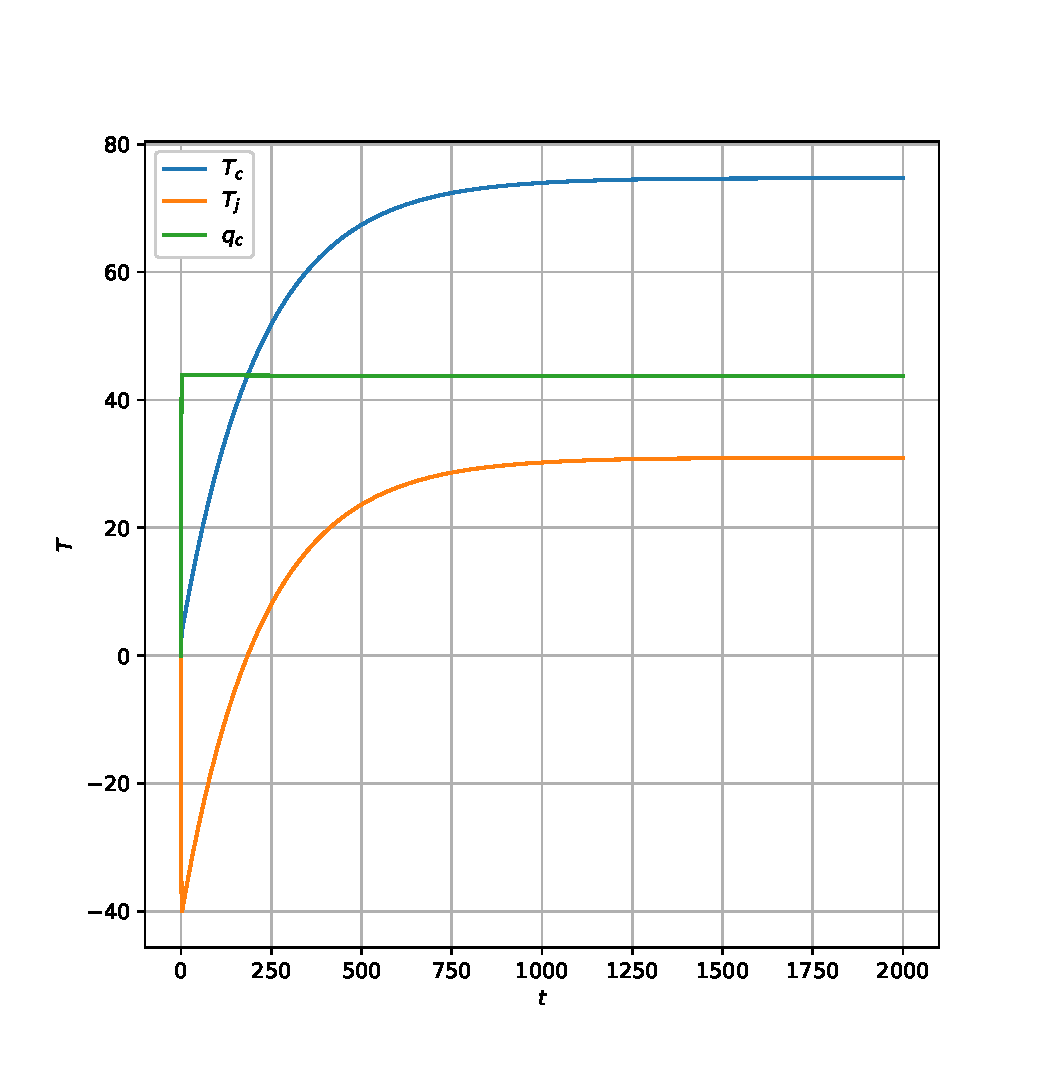
\includegraphics[width=0.50\linewidth]{Images/sin_disipador_step.eps}}
   \subfloat[]{\label{fig:sin_disipador_pulse}
   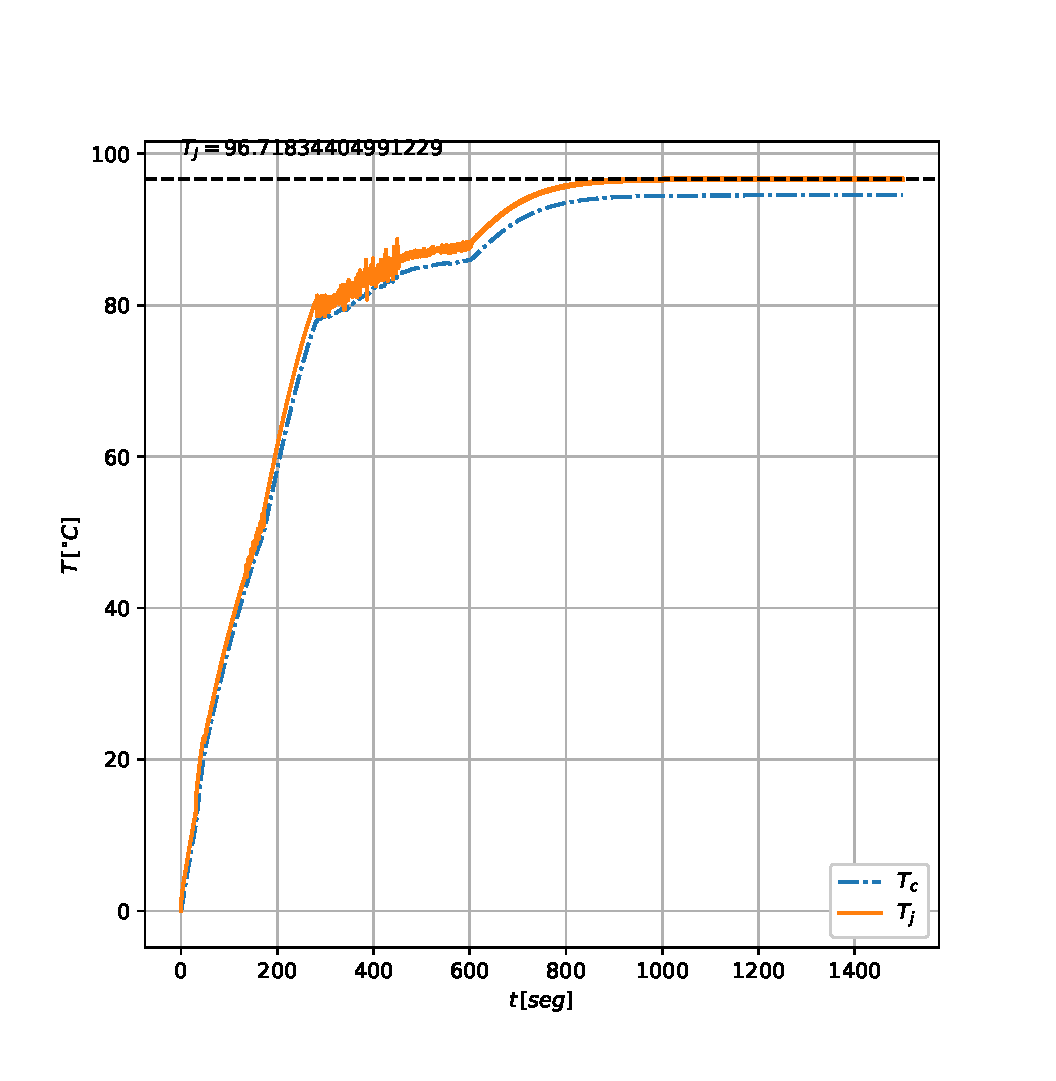
\includegraphics[width=0.50\linewidth]{Images/sin_disipador_pulse.eps}}%[20pt]
   \caption{Respuesta del sistema sin disipador: (a) entrada: escalón (b) entrada: pulsante}
\end{figure}
%------------------------------------------------------------------------------
%                      con disipador graficos simulacion
%------------------------------------------------------------------------------
\begin{figure}[H]
   \centering
   \subfloat[]{\label{fig:con_disipador_step}
   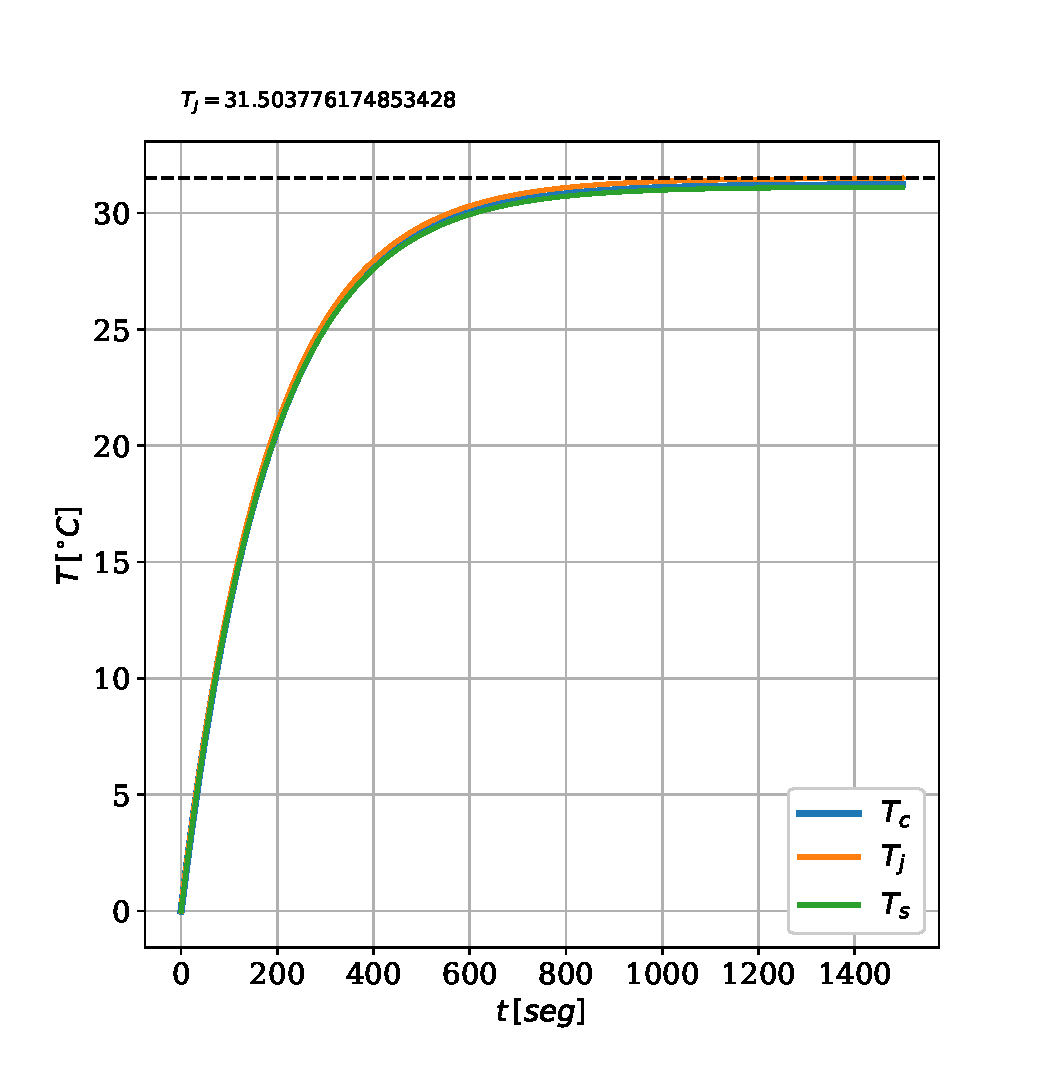
\includegraphics[width=0.50\linewidth]{Images/con_disipador_step.eps}}
   \subfloat[]{\label{fig:con_disipador_pulse}
   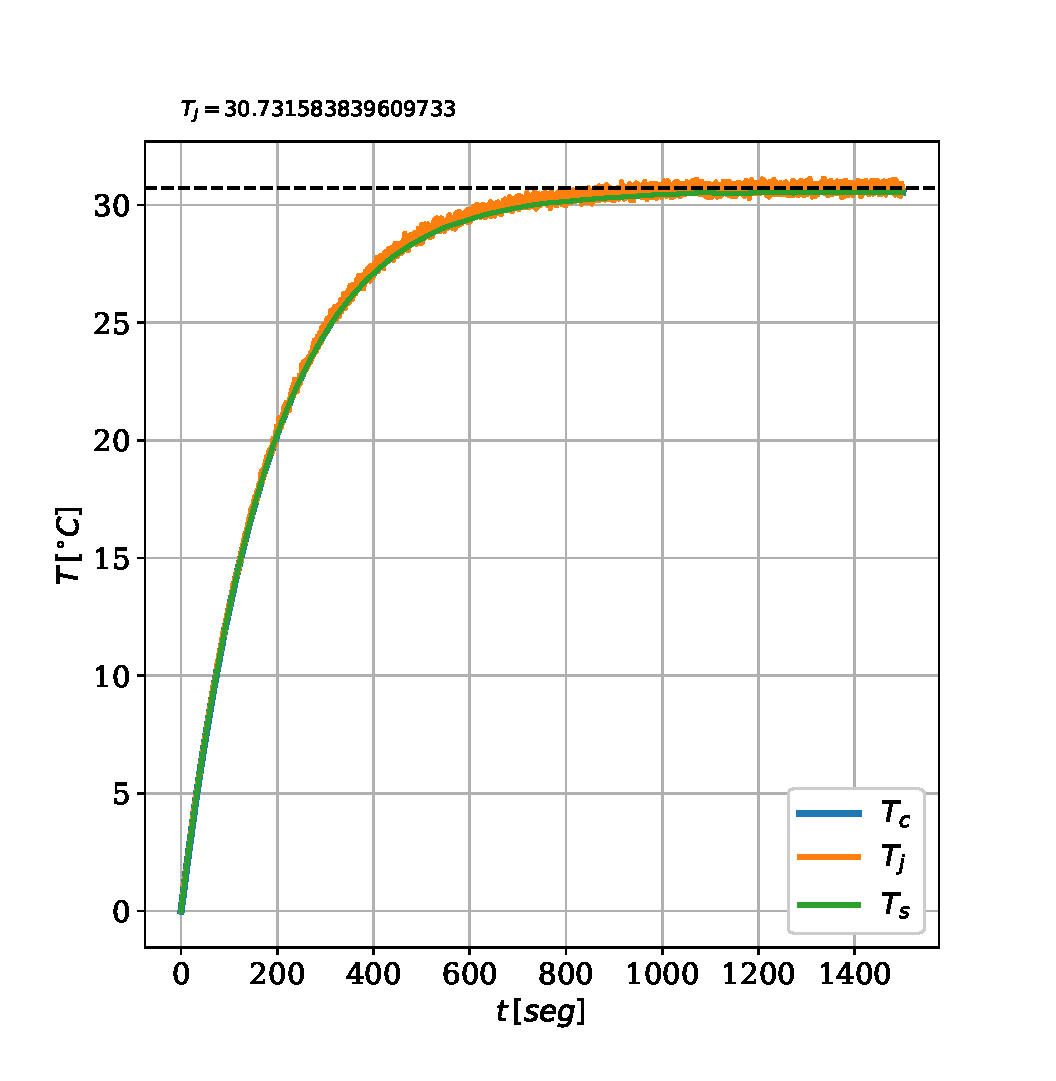
\includegraphics[width=0.50\linewidth]{Images/con_disipador_pulse.eps}}%[20pt]
   \caption{Respuesta del sistema con disipador: (a) entrada: escalón (b) entrada: pulsante}
\end{figure}
%------------------------------------------------------------------------------
%                      conclusiones
%------------------------------------------------------------------------------
\subsection{Conclusiones}
A modo de resumen presentamos la siguiente tabla para representar los resultados:
%------------------------------------------------------------------------------
%                      tabla resumen
%------------------------------------------------------------------------------
\begin{table}[H]
\centering
\caption{resumen de resultados obtenidos}
\label{tabla:resultados1}
\begin{tabular}{|
>{\columncolor[HTML]{9B9B9B}}c |
>{\columncolor[HTML]{FFCCC9}}c |
>{\columncolor[HTML]{FFCCC9}}c |
>{\columncolor[HTML]{FFCCC9}}c |
>{\columncolor[HTML]{FFCCC9}}c |}
\hline
\cellcolor[HTML]{FFFFC7}\textbf{Variable} & \cellcolor[HTML]{C0C0C0}$T_{j_{\max}}[\degree C]$ & \cellcolor[HTML]{C0C0C0}$P_{d_{\max}}^{osc}[W]$ & \cellcolor[HTML]{C0C0C0}$\Delta T_{amb}[\degree C]$ & \cellcolor[HTML]{C0C0C0}tiempo de simulación{[}seg{]} \\ \hline
\textbf{Sin disipador entrada escalon}    & 149.810                                           & 3.870                                           & 119.810                                             & 1500                                                  \\ \hline
\textbf{Sin disipador entrada pulsante}   & 96.718                                            & 38.709                                          & 66.718                                              & 1500                                                  \\ \hline
\textbf{Con disipador entrada escalon}    & 31.503                                            & 16.700                                          & 1.503                                               & 1500                                                  \\ \hline
\textbf{Con disipador entrada pulsante}   & 30.731                                            & 167.001                                         & .731                                                & 1500                                                  \\ \hline
\end{tabular}
\end{table}
%------------------------------------------------------------------------------
%                      fin tabla resumen
%------------------------------------------------------------------------------
De los resultados gráficos y los presentados en [\ref{tabla:resultados1}] vemos que con el uso del disipador se llega a disipar una gran parte del calor generado
por el dispositivo electrónico, con temperaturas máximas muy similares a la temperatura ambiente. Además con el uso del mismo vemos que la potencias máximas
a las que se lo puede someter son significativamente más elevadas que la alternativa sin disipador.
%------------------------------------------------------------------------------
%                      fin problema 1
%------------------------------------------------------------------------------

